% Copyright 2018 Sebastian B. Galkin

% This file is part of paraseba/scaladores-may-2018-talk.

% paraseba/scaladores-may-2018-talk is free software: you can redistribute it and/or modify
% it under the terms of the GNU General Public License as published by
% the Free Software Foundation, either version 3 of the License, or
% (at your option) any later version.

% paraseba/scaladores-may-2018-talk is distributed in the hope that it will be useful,
% but WITHOUT ANY WARRANTY; without even the implied warranty of
% MERCHANTABILITY or FITNESS FOR A PARTICULAR PURPOSE.  See the
% GNU General Public License for more details.

% You should have received a copy of the GNU General Public License
% along with Foobar.  If not, see <http://www.gnu.org/licenses/>.




% Title: Monoids. What, how and why?
% Titulo: Monoides. Que, Como e Por Que?

% Abstract:
% We will learn about Monoids, a concept invented (discovered?) by mathematicians
% that we can leverage to great value in our code and designs.

% The talk is structured in two sessions, in this first one (5/29) we'll learn what
% Monoids are, go through many examples, and write code that creates and uses Monoids. In
% the second session (June maybe?) we will see how we can use Monoids to guide software design.

% Despite the weird name, Monoids are easy to understand, and once you do, you'll
% start finding them everywhere. More importantly, after a little practice
% you'll gain intuition and you'll be able to integrate Monoids in your code and
% designs, obtaining more abstract and reusable results.

% Requirements:
% This is an intermediate level talk. No knowledge of math or functional
% programming is required. I'll assume you can understand simple Scala code.
% In particular, if you don't know what implicit parameters are, spend 10 minutes
% learning about them. You don't need to understand the details of implicit search
% mechanisms or anything like that.


% Resumo:
% Vamos aprender sobre Monoids, um conceito inventado (ou descoberto?) pelos
% matematicos, que nos podemos aproveitar com grandes resultados no nosso codigo e desenhos.

% A palestra esta estruturada em duas sessoes, na primeira (29/05) vamos aprender o
% que sao os Monoids, ver muitos exemplos e escrever codigo que cria e usa
% Monoids. Na segunda sessao (data a confirmar) vamos ver como podemos usar os
% Monoids para guiar o desenho de software.

% Apesar de seu nome estranho, os Monoids sao faceis de entender, e uma vez que os
% entenda, voce vai acha-los em todo lugar. Ainda mais importante, com um
% pouco de pratica, voce vai aprimorar sua intuicao e sera capaz de integrar Monoids no seu
% codigo e desenhos, consiguindo resultados mais abstratos e reusaveis.

% Requerimentos:
% Essa e uma palestra de nivel intermediario. Nao precisa conhecimentos de
% matematica ou programacao funcional. Todos os exemplos serao em Scala, voce devera
% conhecer a linguagem para entende-los. Particularmente, se voce nao sabe o que sao os parametros
% implicitos, gaste 10 minutos aprendedo-os. Nao precisa saber os detalhes dos
% mecanismos de busca de implicitos.

% https://www.theguardian.com/info/developer-blog/2016/dec/22/parental-advisory-implicit-content
% https://docs.scala-lang.org/tutorials/FAQ/context-bounds.html

% Bio:

% Depois de quase uma década trabalhando em linguagens imperativas, Sebastian
% abraçou a programação funcional e nunca mais olhou para atrás. Nos últimos oito anos
% ele tem trabalhado nas áreas de data science, infraestrutura de Big Data e
% enterprise software, em linguagens como Scala, Haskell e Clojure. Cuidado!
% O Sebastian vai tentar trazer você para o mundo da programação funcional.


\documentclass{beamer}
\usepackage[english]{babel}
\usepackage[utf8]{inputenc}
\usepackage[T1]{fontenc}
\usepackage{pgfpages}
\usepackage{listings}
\usepackage{color}
\usepackage{ulem} % for \sout
\usepackage{tikz}
\usepackage{amsmath}
\usepackage{upquote} % make verbatin quotes vertical


\mode<presentation>
{
  \usetheme{Madrid}      % or try Darmstadt, Madrid, Warsaw, ...
  \usecolortheme{default} % or try albatross, beaver, crane, ...
  \usefonttheme{default}  % or try serif, structurebold, ...
  \useoutertheme{default}
  \setbeamertemplate{navigation symbols}{}
  \setbeamertemplate{caption}[numbered]

  % \AtBeginSection[]
  % {
  %   \begin{frame}<beamer>\frametitle{OUTLINE}
  %     \tableofcontents[currentsection,currentsection]
  %   \end{frame}
  % }

}

%\setbeameroption{show notes on second screen}
%\setbeameroption{show only notes}

\setbeamerfont{note page}{size=\tiny}
\setbeamertemplate{note page}[plain]




\title[Monoids]{MONOIDS}
\subtitle{\textit{What}, \textit{How} and \textit{Why}}
\author{Sebastian Galkin}
\institute[@paraseba]{\texttt{@paraseba} \\ \texttt{paraseba@gmail.com}}
\date[Scaladores]{Scaladores - May 2018}
\subject{Talks}

\begin{document}
\lstset{
  language=Scala,
  basicstyle={\small\ttfamily},
  keywordstyle={\usebeamercolor{example text}\color{fg}},
  commentstyle={\usebeamercolor{palette sidebar tertiary}\color{fg!170!}\itshape},
  columns=fullflexible,
  escapechar=~,
  showlines=false,
}


\begin{frame}
  \titlepage
\end{frame}

\begin{frame} \frametitle{OUTLINE}
  \tableofcontents
  \begin{block}{}
    \centering
    \Large \textbf{Ask questions as we go!}
  \end{block}
\end{frame}


\begin{frame} \frametitle{ABOUT ME}
  {\LARGE Sebastian Galkin}

  \begin{itemize}
  \item \alert{Functional Programming} for a while.
  \item Mostly big data and enterprise.
  \item You or your team want to learn more about FP?
    \vspace{4mm}

    {\addtolength{\parindent}{5mm}
      {\addtolength{\parindent}{5mm}
      e-mail: \usebeamercolor{structure}{\textcolor{fg}{\texttt{paraseba@gmail.com}}}

      twitter: \usebeamercolor{structure}{\textcolor{fg}{\texttt{@paraseba}}}
      }
    }
  \end{itemize}
\end{frame}

\section{Abstraction}

\begin{frame} \frametitle{WHAT IS ABSTRACTION?}
  \begin{quote}
\textbf{Abstraction} is the process of extracting the underlying \alert{essence of a concept},
removing any \alert{dependence} on real world objects, and \alert{generalizing} it so that it
has \alert{wider applications.}\\[2ex] \rightline
  {{\rm --- Wikipedia, \href{https://en.wikipedia.org/wiki/Abstraction_(mathematics)}{\underline{Abstraction (mathematics)}}}}
  \end{quote}
\end{frame}


\begin{frame} \frametitle{STANDING ON THE SHOULDERS OF GIANTS}
  Mathematicians are the \alert{masters of abstraction.}
  \begin{itemize}
  \item Maximize generality.
  \item Maximize simplicity (elegance).
  \item Analogies and ``analogies between analogies''.
  \item Reuse whole theories.
  \item Find the right level of abstraction.
  \end{itemize}

  \begin{block}{}
    \centering \Large
    \textbf{They have been doing this for centuries.}
  \end{block}
\end{frame}


\section{What is a Monoid}

\begin{frame} \frametitle{WHAT IS A MONOID?}
  \begin{block}{Components - A triplet \((A, \bullet, u)\)}
  \begin{itemize}
    \item A [carrier] \alert{set} (\(A\))
    \item A binary \alert{operation} (\(\bullet\))
    \item An \alert{element} of the set \(u\)
  \end{itemize}
  \end{block}

  \pause

  \begin{block}{Laws (\(a,b,c \in A\))}

  \begin{description}[Commutativity:]
    \item[Closure:] \(a \bullet b\) is an element of \(A\)
    \item[Associativity:] \((a \bullet b) \bullet c = a \bullet (b \bullet c)\)
    \item[Identity:] \(u \bullet a = a \bullet u \ = a\)
    \item[\sout{Commutativity:}] \(a \bullet b \neq b \bullet a\)
  \end{description}
  \end{block}
  We sometimes say ``\(A\) \emph{has} a monoid''.
\end{frame}


\section{Writing Monoids}

\begin{frame}\frametitle{BASIC MONOIDS IN PROGRAMMING}
  In programming we identify the carrier set with a type.

  \begin{block}{A few monoids}
  \begin{itemize}
    \item<1-> \texttt{Int} under \texttt{(+)} with \texttt{0}.
    \item<1-> \texttt{Int} under \texttt{(*)} with \texttt{1}.
    \item\only<1>{\texttt{Double} under \texttt{(+)} with \texttt{0}?}
         \only<2->{\alert{\sout{\texttt{Double} under \texttt{(+)} with \texttt{0}}}
           \hspace{2em}
      \( (0.1+0.2)+0.3 \neq 0.1+(0.2+0.3)\).}
    \item<3-> \texttt{Boolean} under \texttt{||} with \texttt{False}.
    \item<3-> \texttt{Boolean} under \texttt{\&\&} with \texttt{True}.
    \item<3-> \texttt{Set[A]} under \texttt{union} with \texttt{Set.empty}.
    \item<3-> \texttt{Map[A,B]} under \texttt{(++)} with \texttt{Map.empty}.
  \end{itemize}
  \end{block}

  \visible<3->{There are many more.}
  \end{frame}

\begin{frame}[fragile]\frametitle{MODELING MONOIDS IN SCALA}
  If the type \texttt{A} \emph{has} a monoid we need:
  \begin{itemize}
    \item a way to combine two \texttt{A}s.
    \item a ``special'' value of type \texttt{A} for the identity.
  \end{itemize}
  \pause

  \begin{block}{}
  \begin{lstlisting}
trait Monoid[A] {

  // The associative operation (can't throw)
  def append(a: A, b: => A): A

  // The identity
  def zero: A
}
  \end{lstlisting}
  \end{block}

  We can have more than one monoid for the same \texttt{A}
  \begin{block}{But wait}
    What happened to the laws?
  \end{block}
\end{frame}

\begin{frame}[fragile]\frametitle{OPTIONAL SYNTAX SUGAR}
  \begin{block}{}
  \begin{lstlisting}
import MonoidSyntax._  // assume this in all slides

~\fbox{a |+| b}~ === implicitly[Monoid[A]].append(a,b)  // nicer syntax
  \end{lstlisting}
  \end{block}

  \begin{block}{No need to understand this code}
  \begin{lstlisting}
object Monoid {
  def apply[A:Monoid]: Monoid[A] = implicitly[Monoid[A]]
}

object MonoidSyntax {
  implicit def ToMonoidOps[A:Monoid](v: A) = new MonoidOps[A](v)
  final class MonoidOps[A:Monoid](val self: A) {
    def |+|(other: => A): A = Monoid[A].append(self, other)
  }
}
  \end{lstlisting}
  \end{block}
\end{frame}

\begin{frame}[fragile]\frametitle{TWO MONOIDS FOR \texttt{Int}}
  \begin{block}{}
  \begin{lstlisting}
val intAddMon = new Monoid[Int] {

  def append(a: Int, b: => Int): Int =
    a + b

  def zero: Int = 0
}

val mulMon = new Monoid[Int] {

  def append(a: Int, b: => Int): Int =
    a * b

  def zero: Int = 1
}
  \end{lstlisting}
  \end{block}
  Monoids \alert{instances} are first class citizens.
\end{frame}

\begin{frame}[fragile]\frametitle{THE LIST MONOID}
  \begin{block}{}
    List[Int](1, 2, 3, 4) |+| List[Int](5, 6, 7, 8) = List[Int](???)
  \end{block}

  \pause

  \begin{block}{A default (?) monoid for Lists}
  \begin{lstlisting}

implicit def freeMon[A]: Monoid[List[A]] = new Monoid[List[A]] {

  def append(as: List[A], bs: => List[A]): List[A] =
    as ++ bs

  def zero: List[A] = List()
}
  \end{lstlisting}
  \end{block}
  Our first noncommutative monoid.
\end{frame}

\begin{frame}[fragile]\frametitle{MONOID FOR TUPLES}
  How can we combine two tuples \texttt{(A,B)}:

  \begin{block}{}
  \begin{lstlisting}
(4, List('H','e','l','l','o')) |+| (2, List('W','o','r','l','d'))
  \end{lstlisting}
  \end{block}

  \pause

  If \texttt{A} and \texttt{B} have monoids themselves, we can \alert{combine componentwise}.

  \begin{block}{}
  \begin{lstlisting}
implicit def pairMon[A: Monoid, B: Monoid] = new Monoid[(A, B)] {
  /* ~\phantom{cit def pairMon[A: Mon}\rotatebox[origin=c]{90}{$\Rsh$}~ syntax sugar for:
     (implicit am: Monoid[A], implicit bm: Monoid[B]) */

  def append(x: (A, B), y: => (A, B)): (A,B) =
    (x._1 |+| y._1, x._2 |+| y._2)

  def zero: (A,B) =
    (Monoid[A].zero, Monoid[B].zero)
}
  \end{lstlisting}
  \end{block}
\end{frame}


\begin{frame}[fragile] \frametitle{A MONOID FOR FUNCTIONS}
  \texttt{Monoid[A => B]} \pause where \alert{\texttt{B} has a monoid}

  \begin{block}{Functions that return a monoidal type}
  \begin{lstlisting}
implicit def monFunMon[A, B:Monoid]: Monoid[A => B] =
  new Monoid[A => B] {

    def zero: A => B =
      _ => Monoid[B].zero

    def append(f: A => B, g: => (A => B)): A => B =
      a => f(a) |+| g(a)
}
  \end{lstlisting}
  \end{block}
  Convince yourself it is a lawful monoid.

  Is it commutative?
\end{frame}


\begin{frame} \frametitle{RECAP}
  We have seen:
  \begin{itemize}
    \item Monoid definition (binary assoc operation with identity).
    \item Monoid \texttt{trait} (one type parameter,
      two methods: \texttt{zero, append}).
    \item Monoids for:
      \begin{itemize}
      \item Numbers, lists, tuples (if components have monoids).
      \item \texttt{A => M} where \texttt{M} has a monoid.
      \item There are many, many more.
      \end{itemize}
  \end{itemize}

  \begin{block}{}
    \centering
    But \alert{why} or \alert{how} to use monoids.
  \end{block}
\end{frame}

\section{Usage}
\begin{frame}[fragile] \frametitle{SIMPLE USAGE EXAMPLES}
  \framesubtitle{\texttt{mconcat}}

  \begin{block}{A useful little function}
  \begin{lstlisting}
// (a1 |+| a2) |+| a3 === a1 |+| (a2 |+| a3)
def mconcat[A:Monoid](as: Traversable[A]): A =
  as.foldLeft(Monoid[A].zero)(_ |+| _)
  // === as.foldRight(Monoid[A].zero)(_ |+| _)~\pause~

def sum(xs: Traversable[Int]): Int =
  ~\alert{mconcat}~(xs)(intAddMon)

def concat[A](xs: Traversable[List[A]]): List[A] =
  ~\alert{mconcat}~(xs)(freeMon) // or get the Monoid implicitly
  \end{lstlisting}
  \end{block}
\end{frame}

\begin{frame}[fragile] \frametitle{SIMPLE USAGE EXAMPLES}
  \framesubtitle{Functional MapReduce}
  \begin{block}{Super useful: \texttt{foldMap}}
  \begin{lstlisting}
def foldMap[A, M:Monoid](as: Traversable[A], f: A => M): M =
  //  === mconcat(as.map(f))

  as.foldLeft(Monoid[M].zero) { _ |+| f(_) }
  \end{lstlisting}
  \end{block}

  \texttt{f} acts as the mapping phase in a MapReduce, the monoidal
  operation is the reduction step.

  \begin{block}{}
  \begin{lstlisting}
def filter[A](as: List[A], f: A => Boolean): List[A] =
  foldMap(as, (a:A) =>
    if (f(a)) List(a)
    else List())(freeMon)
  \end{lstlisting}
  \end{block}
\end{frame}


\begin{frame}[fragile] \frametitle{COMPOSING MONOIDS}
  \framesubtitle{A monoid to compute min/max}
  \begin{block}{A monoid for minimum}
  \begin{lstlisting}
def minMon[A:Ordering]: Monoid[Option[A]] =
  new Monoid[Option[A]] {~\pause~

    def append(a: Option[A], b: => Option[A]): Option[A] =
      (a, b) match {
        case (None, x) => x
        case (x, None) => x
        case (Some(x), Some(y)) => Some(Ordering[A].min(x,y))
      }

    def zero: Option[A] = None
}
  \end{lstlisting}
  \end{block}
  We can do the same for \texttt{maxMon}.
\end{frame}


\begin{frame}[fragile] \frametitle{COMPOSING MONOIDS}
  \framesubtitle{A monoid to compute min/max}
  \begin{block}{Calculate \texttt{min} \& \texttt{max} in a \alert{single pass}}
  \begin{lstlisting}
def min[A: Ordering](as: Traversable[A]): Option[A] =
  foldMap(as, (a:A) => Option(a))(minMon) // map and reduce ~\pause~

def minMaxMon[A:Ordering] = ~\alt<2,3>{\alert{???}}{\alert{pairMon(minMon, maxMon)}}~

def minmax[A: Ordering](as: Traversable[A]): Option[(A,A)] =  ~\pause~
  foldMap(as, (a:A) => (Option(a), Option(a)))(minMaxMon) match {

    case (Some(mi), Some(ma)) => Some((mi,ma))
    case _ => None
  }
  \end{lstlisting}
  \end{block}

  \visible<4->{
  \begin{itemize}
    \item Note how easily the monoids \alert{compose}.
    \item Can be extended to other \alert{aggregates} \texttt{(min, max, sum, size)}.
  \end{itemize}
  }
\end{frame}

\begin{frame} \frametitle{POWERFUL ABSTRACTION}
  \textbf{\large Monoids compose extremely well.}
  \begin{itemize}
    \item \texttt{A: Monoid}
    \item \texttt{B: Monoid}
      \pause
    \item \texttt{Option[B]: Monoid}
      \pause
    \item \texttt{(A, Option[B]): Monoid}
    \item \texttt{List[(A, Option[B])]: Monoid}
      \pause
    \item \texttt{Y => List[(A, Option[B])]: Monoid}
      \pause
    \item \texttt{X => Y => List[(A, Option[B])]: Monoid}
    \item \texttt{Map[String, X => Y => List[(A, Option[B])]]: Monoid}
  \end{itemize}

  \textbf{\large Monoids are very expressive.}
  \pause
  \begin{itemize}
    \item \texttt{mconcat: sum, concat, ...}
    \item \texttt{foldMap: fold*, filter, map, ...}
  \end{itemize}

  \begin{block}{}
    \centering
    \Large \textbf{Signs of a good abstraction}
  \end{block}
\end{frame}

\begin{frame} \frametitle{LARGER USE CASES}
  \framesubtitle{Parallelization}
  \begin{block}{The problem}
    \begin{itemize}
      \item Merge multiple renders into one.
      \item \texttt{merge} is an expensive operation.
      \item \texttt{merge(img1, merge(img2, merge(img3, ...)))}
      \item Obvious solution: \texttt{mconcat( List(img1, img2, ..., imgn) )}
    \end{itemize}
  \end{block}

  \pause
  \begin{center}
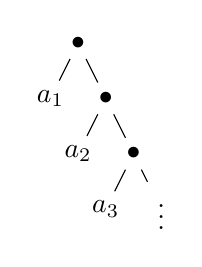
\begin{tikzpicture}[sibling distance=2em, level distance=2em]
  \node {\(\bullet\)}
    child { node {\(a_1\)} }
    child { node {\(\bullet\)}
      child { node {\(a_2\)}}
      child { node {\(\bullet\)}
        child { node {\(a_3\)}}
        child { node {\(\vdots\)}
    }}};
\end{tikzpicture}
\qquad
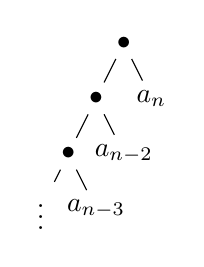
\begin{tikzpicture}[sibling distance=2em, level distance=2em]
  \node {\(\bullet\)}
    child { node {\(\bullet\)}
      child { node {\(\bullet\)}
        child {node {\(\vdots\)}}
        child {node {\(a_{n-3}\)}}}
      child { node {\(a_{n-2}\)}}
        }
    child { node {\(a_n\)} };
\end{tikzpicture}
\qquad
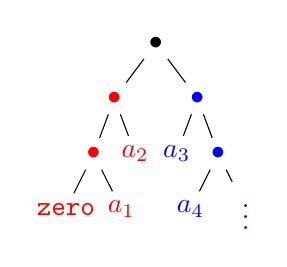
\begin{tikzpicture}[level distance=2em, level 3/.style={sibling distance=2em}, level 2/.style={sibling distance=1.5em}, level 1/.style={sibling distance=3em}]
  \node {\(\bullet\)}
  child { node[color=red] {\(\bullet\)}
    child { node[color=red] {\(\bullet\)}
      child {node[color=red] {\texttt{zero}}}
      child {node[color=red] {\(a_1\)}}}
    child { node[color=red] {\(a_2\)}}
  }
  child { node[color=blue] {\(\bullet\)}
    child { node[color=blue] {\(a_3\)} }
    child { node[color=blue] {\(\bullet\)}
      child { node[color=blue] {\(a_4\)}}
      child { node[color=blue] {\(\vdots\)}
      }}};
\end{tikzpicture}
\end{center}
\end{frame}

\begin{frame}[fragile] \frametitle{LARGER USE CASES}
  \framesubtitle{Parallelization}

  \begin{block}{}
  \begin{lstlisting}
object Parallel {

  def mconcat[A:Monoid](as: Traversable[A]): A =
    ~\alt<1>{as.foldLeft(Monoid[A].zero)(\_ |+| \_)}{}\alt<2>{as.\alert{fold}(Monoid[A].zero)(\_ |+| \_)}{}\alt<3->{as.\usebeamercolor{structure}\textcolor{fg}{par}.\alert{fold}(Monoid[A].zero)(\_ |+| \_)}{}~
}
  \end{lstlisting}
  \end{block}

  \invisible<1>{
    \texttt{fold[A1 >: A](z: A1)(op: (A1, A1) => A1): A1}
    \vspace{2ex}

    \texttt{z}: a \alert{neutral} element for the fold operation;
    may be added to the result an arbitrary number of times, and \alert{must not change the result.}

    \texttt{op}: a binary operator that must be \alert{associative.}
    \begin{block}{}
      \centering
      \large \textbf{That's just a monoid!}
    \end{block}
  }
\end{frame}

\begin{frame} \frametitle{LARGER USE CASES}
  \framesubtitle{Incremental updates}
  \begin{block}{The problem}
    \begin{itemize}
      \item System measures request latency.
      \item \alert{compute} and store \alert{mean} and \alert{variance.}
      \item Events arrive at high rate, \alert{millions per hour.}
    \end{itemize}
  \end{block} \pause
  \begin{columns}[c]
    \column{0.6\textwidth}
      \begin{block}{Naive approach}
        \begin{itemize}
        \item Store all measurements,
        \item compute \(\mu, \sigma^2\) on demand, or
          precompute at certain interval.
        \end{itemize}
      \end{block}

    \column{0.3\textwidth}
  Too much \alert{space}, too much \alert{time}. \(\mathcal{O}(N)\).
  \end{columns}
\end{frame}

\begin{frame} \frametitle{LARGER USE CASES}
  \framesubtitle{Incremental updates}
  \begin{block}{A better approach}
  \begin{itemize}
    \item Find a \alert{monoid} to combine \alert{mean/variance} of \(n\) samples.
    \item Store only the stats, not the measurements.
    \item Accumulate several (or 1) new measurements.
    \item \alert{Combine} the old and new stats using the monoid.
    \item Store.
  \end{itemize}
  \end{block}

  \begin{block}{How is it better?}
  \begin{itemize}
    \item \alert{Exact} if we can find the right monoid.
    \item \alert{\(\mathcal{O}(1)\) updates} (independent of sample size).
    \item Trade off freshness by scale.
  \end{itemize}
  \end{block}
\end{frame}

\begin{frame} \frametitle{LARGER USE CASES}
  \framesubtitle{Incremental updates}
  What does the monoid need?
  \begin{block}{Weighted average of the means}
    \[
    \begin{split}
      n\cdot \mu = \sum_{i=0}^{n-1} x_i \qquad  m\cdot \nu = \sum_{i=0}^{m-1} x_{i+n} \\
      \frac{1}{n+m} \sum_{i=0}^{n+m-1} x_i = \frac{\alert{n}\cdot\mu + \alert{m}\cdot\nu} {\alert{n+m}}
    \end{split}
    \]
  \end{block}

  We need previous \alert{mean} and \alert{sample size.}

  Generalizing, to compute the nth-moment, we need to store n+1 values.
\end{frame}

\begin{frame}[fragile] \frametitle{LARGER USE CASES}
  \framesubtitle{Incremental updates}
  \begin{block}{A data type for mean and variance}
  \begin{lstlisting}
sealed abstract class MeanVar

final case object EmptyMeanVar extends MeanVar

final case class MeanVarV(
  m1: Double,
  m2: Double,
  n: Long) extends MeanVar
  \end{lstlisting}
  \end{block}
\end{frame}

\begin{frame}[fragile] \frametitle{LARGER USE CASES}
  \framesubtitle{Incremental updates}
  \begin{block}{The MeanVar monoid}
  \begin{lstlisting}
val meanVarMonoid: Monoid[MeanVar] = new Monoid[MeanVar] {
  def zero: MeanVar = EmptyMeanVar

  def append(a: MeanVar, b: => MeanVar): MeanVar = (a, b) match {
    case (EmptyMeanVar, a) => a
    case (a, EmptyMeanVar) => a ~\pause~

    case (MeanVarV(m1a, m2a, na), MeanVarV(m1b, m2b, nb)) => {
      val (nt, delta) = (na + nb, m1b - m1a)
      MeanVarV(~\alert{(na * m1a + nb * m1b ) / nt}~,
                m2a + m2b + delta * delta * na * nb / nt,
                ~\alert{nt}~)
    }
  }
  \end{lstlisting}
  \end{block}
\end{frame}

\begin{frame}[fragile] \frametitle{LARGER USE CASES}
  \framesubtitle{Incremental updates}
  \begin{block}{Utility functions: creating \texttt{MeanVars}}
  \begin{lstlisting}
object MeanVar {

  def singleton(x: Double): MeanVar = MeanVarV(x, 0, 1)

  def sample(xs: Traversable[Double]): MeanVar = ~\pause~
    foldMap(xs, singleton)  // === mconcat(xs.map(singleton))
}
  \end{lstlisting}
  \end{block}
\end{frame}

\begin{frame}[fragile] \frametitle{LARGER USE CASES}
  \framesubtitle{Incremental updates}
  \begin{block}{Updating the statistics (pseudocode)}
  \begin{lstlisting}
     // Define a time resolution (accumulate for 1sec? 100ms?)
     val newSample: Vector[Double] = getNewMeasurements(...)

     // Compute mean/var of the new data (incremental work)
     val newStats: MeanVar = MeanVar.sample(newSample)

     // This is an O(1) op
     // In our example this loads 3 numbers,
     // doesn't matter how many samples we have processed before
     val oldStats: MeanVar = loadStats(...)

     // Another O(1) operation
     storeStats(oldStats |+| newStats)
  \end{lstlisting}
  \end{block}
\end{frame}


\begin{frame} \frametitle{LARGER USE CASES}
  \framesubtitle{Incremental updates}
  \begin{block}{Notice:}{}
  \begin{itemize}
    \item We never wrote the alg. to compute mean/var, only to combine them.
    \item Extensible to higher momenta.
    \item Extensible to approximate histograms and other fun stuff.
    \item Didn't we say \texttt{Double} under \texttt{(+)} is not a monoid?
  \end{itemize}
  \end{block}
\end{frame}

\begin{frame} \frametitle{CONCLUSIONS}
  \begin{itemize}
    \item You could have \emph{invented} the monoid.
    \item You could have \emph{discovered} the laws.
    \item Write only \alert{lawful} monoids.
    \item \alert{Use the monoid}. They are everywhere.
    \item Don't be afraid of other algebraic structures (Functor, Monad).
    \item \alert{Learn how to abstract}, copy and steal.
  \end{itemize}
\end{frame}

\section*{References}
\begin{frame} \frametitle{REFERENCES}
  \begin{columns}[c]
    \column{0.7\textwidth}
      \begin{itemize}

        \item This talk: slides, all the \alert{code and many tests} \\
          \href{https://github.com/paraseba/scaladores-may-2018-talk}{\scriptsize \underline{\texttt{https://github.com/paraseba/scaladores-may-2018-talk}}}

        \item \textit{Functional Programming in Scala}\\ Paul Chiusano \& Runar Bjarnason

        \item \textit{Why Functional Programming Matters} \\
          John Hughes.

        \item Scalaz library \\
          {\href{https://github.com/scalaz/scalaz}{\scriptsize\underline{\texttt{https://github.com/scalaz/scalaz}}}}

        \item \textit{Computing skewness and kurtosis in one pass} \\
          {\footnotesize
            \href{https://www.johndcook.com/blog/skewness\_kurtosis/}{\scriptsize\underline{\texttt{https://www.johndcook.com/blog/skewness\_kurtosis/}}}}
      \end{itemize}

    \column{0.3\textwidth}

    \begin{figure}
        \vspace{10ex}
        \centering
        \includegraphics[width=\textwidth]{functional-programming-in-scala.png}
    \end{figure}
  \end{columns}
\end{frame}

% \begin{frame}{ToDo / Fixme}
%   \begin{itemize}
%     \item topic for design session: aggregations (a la beautiful folds)
%     \item topic for design session: diagrams library design
%   \end{itemize}
% \end{frame}

\end{document}